\documentclass[../documentation.tex]{subfiles}
 
\begin{document}

\section{Irodalomkutatás}
\subsection{Ipar 4.0 eredete}
Az Ipar 4.0 koncepcióját Németországban dolgozták ki, ahol világszinten kiemelkedő a termelési iparág, illetve világvezető a gyártó eszközök területén. Az Ipar 4.0 a német kormány stratégiai kezdeményezése volt, mely nagy mértékben támogatta az ipari szektor fejlesztését. Ilyen értélemben az Ipar 4.0-ra tekinthetünk egy olyan mozgalomként, amelynek célja megőrizni Németország befolyását a gépiparban és az autógyártás területén.\cite{industry40}

Az alap koncepciót először a Hanover Fair-en\footnote{A hannoveri a világy egyik legnagyobb kereskedelmi bemutatója. Körülbelül 6500 kiállító és 250.000 látogató vesz részt ezen a rendezvényen.} prezentálták 2011-ben. A bemutató óta az Ipar 4.0 Németország vezető témája a kutatások területén, egyetemi és ipari környezetekben különféle eseményeken. A fő irányvonal az új technológiákban és koncepciókban rejlő potenciál kihasználása felé mutat, ilyen területek:
\begin{itemize}
	\item az IoT (\foreignlanguage{british}{Internet of Things}\footnote{A Dolgok internete fizikai eszközökből, járművekből, otthoni felszerelésekből és további elektronikát, szoftvert, szenzorokat, aktuátorokat tartalmazó tételekből álló hálózat, amelyek képesek egymással kapcsolatba lépni, adatot fogadni és küldeni.}) elérhetősége és kihasználása,
	\item a technológiai és gazdasági folyamatok integrációja cégen belül,
	\item a valóság virtuális leképezése,
	\item `okos' gyárak beleértve az `okos' gyártást és termékeket.
\end{itemize}

\subsection{Előnyei}
Amellett hogy a digitalizáció és az új technológiák természetes következménye, az Ipar 4.0 megjelenése szintén kapcsolatban áll azzal a ténnyel, hogy a gyártásban a profit nővelésére irányuló kezdeményezések, lehetőségek nagy része kiaknázásra került, új megoldásokat kellett keresni. A gyártási költségek csökkentek a Just-In-Time (röviden JIT) termelés bevezetésével, a lean elveinek alkalmazásával és a gyárak olyan helyre telepítésével, ahol a munkaerő lényegesen olcsóbb. Ha az előállítási költségek minimalizálása a célunk, az Ipar 4.0 egy ígéretes megoldásnak tűnik. Számos forrás alapján az Ipar 4.0 alkalmazása csökkentheti\cite{industryresults}:
\begin{itemize}
	\item a gyártás költségét 10-30\%-kal,
	\item a logisztikával kapcsolatos kiadásokat 10-30\%-kal,
	\item a minőségmenedzsmenthez köthető költségeket 10-20\%-kal.
\end{itemize}

Ezeken kívűl a koncepció alkalmazásának számos egyéb előnyéről szólhatunk: (1) új termékek piacra kerülési ideje csökken, (2) érzékenyebb reagálás a megváltozott vásárlói igényekre, (3) lehetővé teszi a személyreszabott tömeggyártást az össz gyártási költség jelentős növelése nélkül, (4) rugalmasabb és barátságosabb munkakörnyezetet teremt, (5) a természetes erőforrásokat hatékonyabban hasznosítja.

%============================================================
\subsection{Kialakítási alapelvek}
A számos szövegelemzés és átfogó irodalmi áttekintés négy fő dizájn elvet emelt ki, hogy irányvonalat mutasson a szakértőknek és tudósoknak az Ipar 4.0 környezet kialakításához: összekötés, információs átláthatóság, decentralizált döntéshozatal és technikai asszisztens (\ref{fig:designprinciples}. ábra). Ezek az alapelvek a következő alfejezetekben kerülnek részletes tárgyalásra az egyetemi és ipari publikációkban használt kifejezések (és következésképpen a kialakítási alapelvek) rövid elemzése után.

Összességében a két különböző típusú publikáció szövegelemzése nem mutat lényeges eltérést, mindkettő típus külön-külön elemzése ugyanazokat a kialakítási alapelveket eredményezi. Azonban szembe tűnő, hogy egyes dizájn elemeket gyakrabban tárgyalnak a gyakorlati publikációkban. Az ember-robot kollaboráció, adat- és információbiztonság és a decentralizált döntéshozatal gyakrabban fordul elő ipari kiadványokban. Az első kettővel kapcsolatos értekezések magas száma rávilágít az Ipar 4.0 eredményes implemetálásának legnagyobb kihívásaira amivel az iparban dolgozók szembesülnek. Mindeközben a decentralizált döntéshozatalt tekintik az Ipar 4.0 legproblémásabb elemének, és ezért ez rendkívül részletes és átfogó tárgyalásra kerül.

\begin{figure}
\centering
\begin{tikzpicture}
[node distance = 1cm, auto,font=\footnotesize,
% STYLES
every node/.style={node distance=3cm},
% The comment style is used to describe the characteristics of each force
comment/.style={rectangle, inner sep= 5pt, text width=4cm, node distance=0.25cm, font=\scriptsize\sffamily},
% The force style is used to draw the forces' name
force/.style={rectangle, draw, fill=black!10, inner sep=5pt, text width=4cm, text badly centered, minimum height=1.2cm, font=\bfseries\footnotesize\sffamily}] 

% Draw forces
\node [force] (design) {Ipar 4.0\\ Tervezési alapelvek};
\node [force, above of=design] (interconnection) {Összekapcsolás};
\node [force, left=1cm of design] (assistant) {Technikai asszisztens};
\node [force, right=1cm of design] (decentralized) {Decentralizált döntéshozatal};
\node [force, below of=design] (transparency) {Információs átláthatóság};

% ASSISTANT
\node [comment, below=0.25cm of assistant] {Virtuális asszisztens\\
Fizikai asszisztens};

% INTERCONNECTION
\node [comment, right=0.25 of interconnection] {Együttműködés\\ Szabvány\\ Biztonság};

% TRANSPARENCY
\node [comment, below=0.25 of transparency] {Adatelemzés\\ Információszolgáltatás};

%%%%%%%%%%%%%%%%

% Draw the links between forces
\path[-,thick] 
(design) edge (interconnection)
(design) edge (assistant)
(design) edge (decentralized)
(design) edge (transparency);

\end{tikzpicture} 
\caption{Ipar 4.0 tervezési szempontok}
\label{fig:designprinciples}
\end{figure}

\subsubsection{Összekapcsolás}
Gépek, eszközök, szenzorok és emberek kapcsolatba lépnek IoT-n (\foreignlanguage{british}{Internet of Things} - Dolgok internete) és IoP-n (\foreignlanguage{british}{Internet of People} - Emberek internete\cite{iop}) keresztül és így formálnak egy IoE-t (\foreignlanguage{british}{Internet of Everything} - Minden internete\cite{ioe}). A vezetéknélküli technológiák kiemelkedő szerepet játszanak az interakciók során, mivel lehetővé teszik az internetes hozzáférést mindenfelé. Az IoE-n keresztül összekötött emberek és eszközök képesek egymással információt megosztani, ami a kollaboráció alapját jelenti a közös célok elérése érdekében. 3 különböző típust különböztethetünk meg az IoE kapcsán: ember-ember együttműködés, \textbf{ember-robot kollaboráció} és robot-robot kollaboráció.\cite{collabtypes}

A különböző gépek, eszközök, érzékelők és emberek egymás közti interakciója során elengedhetetlen szerepe van a széles körben elfogadott kommunikációs szabványoknak. Ezek teszik lehetővé a különböző gyártóktól érkező moduláris eszközök rugalmas kombinálását. Ez a modularizáció az alapfeltétel, hogy az Ipar 4.0 `okos' gyárai alkalmazkodni tudjanak a folyamatosan változó piaci igényekhez vagy a személyreszabott rendelésekhez.

Ahogy nő az IoE-ben részt vevők száma, a monetáris\footnote{pénzhez vagy valutához kötődő} és politikai érdekek meg fogják növelni az ilyen létesítmények elleni káros támadások számát, így az igény is nőni fog a magasabb fokú informatikai biztonság iránt.

\subsubsection{Információs átláthatóság}
Az összekapcsolt objektumok és emberek növekvő számának köszönhetően, a fizikai és a virtuális világ egybeolvadása lehetővé tesz egy újfajta információs modellt\cite{newinformation}. Az érzékelők összekapcsolása révén képezhetünk egy digitális, virtuális leképezést a világunkról.

Az összefüggés-tudatos információ az IoE résztvevői számára elengedhetetlenek a megfelelő döntések meghozatalához. Az ilyen összefüggés-tudatos rendszerek a feladataikat virtuális és a fizikai világból érkező iformációk alapján látják el. A virtuális világból érkező információkra példák az elektronikus dokumentumok, rajzok, szimulációs modellek. A fizikai világ információi például a pozíció vagy a szerszám állapota. A fizikai világ elemzéséhez az érzékelők felől érkező nyers adatokat magasabb szintű értelmezési és egyéb információval kell kiegészíteni. Ahhoz, hogy az átláthatóságot fenntartsuk, az adatelemzés eredményeit egy olyan kisegítő rendszerbe kell bevinni, ami minden IoE résztvevő számára elérhető. A folyamatkritikus információk esetén a valós idejű adatszolgáltatás elengedhetetlen.

\subsubsection{Decentralizált döntéshozatal}
A decentralizált döntések meghozatalának két alappilére az ojektumok és emberek összekapcsolása, illetve a termelő létesítményen belülről és kívülről érkező információk átláthatósága. Az összekapcsolt és decentralizált döntéshozó egységek lehetővé teszik a lokális információk globálissal együtti felhasználását egyazon időben, így elősegítve az átgondoltabb döntéshozatalt és így növelve összességében a termelékenységet. Az egyes IoE elemek a feladataikat annyira önállóan látják el, amennyire csak lehet. A feladatok csak kivételek, zavarok vagy ellentmondásos célok esetén kerülnek továbbításra magasabb szintre.

Gyakorlati szempontból a decentralizált döntéshozatalt a kiber-fizikai rendszerek teszik lehetővé. Ezek beágyazott számítóegységeinek, szenzorainak és aktuátorainak felhasználásával történik fizikai világ autonóm nyomon követése és az irányítása.  

\subsubsection{Technikai asszisztens}
Az Ipar 4.0 `okos' gyáraiban az ember szerepe alapvetően megváltozik, gépkezelő helyett inkább stratégiai döntéshozóvá és rugalmas problémamegoldóvá válik. A termelési folyamatok növekvő komplexitása miatt, ahol a kiber-fizikai rendszerek összetett hálózatot alkotnak és decentralizált döntéseket hoznak, az embereknek támogató rendszerekre van szükségük. Ezeknek a rendszereknek a szerepe az információk összegyűjtése és megjelenítése egyértelműen és érthetően annak érdekében, hogy az emberek jól megalapozott döntéseket tudjanak hozni, és magas prioritású problémákat tudjanak megoldani rövid időn belül. Jelenleg az embereket főként az okostelefonjaik és táblagépeik kötik össze az IoT-vel\cite{fromiot2ioe}. A hordozhatóság kiemelkedően fontossá fog válni a jövőben amint a jelenlegi kihívásokon (mint például az energiaellátás) sikerül felülkerekedni.

Az emberek robotok általi fizikai kisegítése (a robotika területen elért fejlesztésekkel) szintén a technikai asszisztens szerep részét képezi. A robotok számos feladatot képesek elvégezni, amelyek az ember számára kellemetlenek, túl fárasztóak vagy veszélyesek más munkásokra nézve\cite{hri}. Az emberek fizikai feladatokban hatékony, sikeres és biztonságos segítésének érdekében szükséges, hogy a robotok az ember társaikkal zökkenőmentesen és intuitívan működjenek együtt\cite{hri}. Ezen felül elengedhetetlen, hogy az emberek megfelelő képzésben részesüljenek az adott ember-robot kollaborációhoz\cite{m-learning}.

\subsection{Ember-robot kollaboráció}
\subsubsection{Fogalmak tisztázása}
Az ember és a robot közösen végzett feladataikat különböző interakciós szinteken valósíthatják meg, ezeket érdemes egymástól elhatárolni\footnote{Forrás: https://hohmannchris.wordpress.com/2017/02/08/cobots-more-cooperation-than-collaboration/} (\ref{fig:coex-coop-collab}. ábra):
\begin{enumerate}
	\item Robot cella (\angol{Robotic cell}): a robot önállóan végzi a feladatát az embertől kerítéssel elválasztva. Ez esetben nem beszélhetünk ember-robot együttműködésről.
	\item Együttes jelenlét (\angol{Coexistence}): a robot és az ember közel helyezkedik el egymáshoz védőkerítés nélkül, de nincs közös munkaterük. A robotnak van saját meghatározott tere.
	\item Szinkronizált munkavégzés (\angol{Synchronized work}): olyan elrendezés, melyben az ember és a robot osztozik egy közös munkateren, de egyszerre csak egyikük aktív. A munkamenet az ember és a robot jól definiált `koreográfiája'.
	\item Kooperáció (\angol{Cooperation}): a két ``partner'' mindegyike a saját feladatával foglalkozik. A munkaterük lehet közös, de nem dolgozhatnak sem ugyanazon a terméken, sem ugyanazon a munkadarabon.
	\item Kollaboráció (\angol{Collaboration}): olyan elrendezés, amely esetén az ember és a robot közösen és szimultán dolgozik egyazon terméken vagy munkadarabon. Tipikusan a robot megfogja, átnyújtja és tartja a munkadarabot amíg a munkás dolgozik rajta.
\end{enumerate}

\begin{figure}[h]
	\centering
	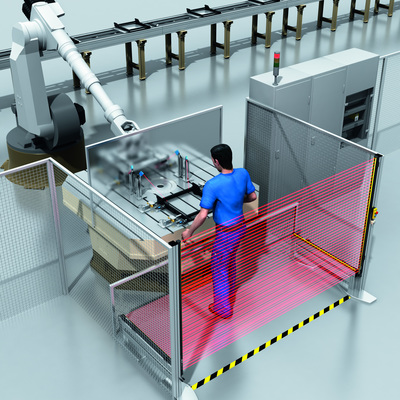
\includegraphics[scale=1.4]{coexistence}
	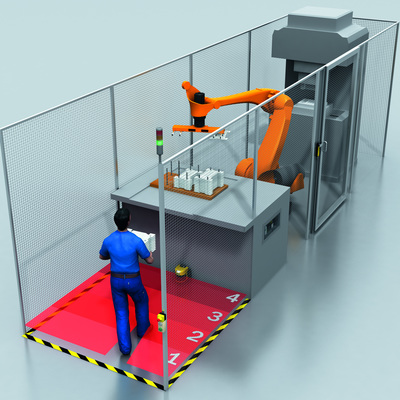
\includegraphics[scale=1.4]{cooperation}
	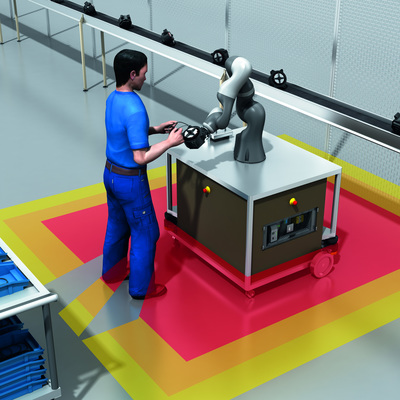
\includegraphics[scale=1.4]{collaboration}
	\caption[Caption for LOF]{Balról jobbra: együttes jelenlét, kooperáció, kollaboráció\footnotemark}
	\label{fig:coex-coop-collab}
\end{figure}

\footnotetext{Képek forrása: https://www.safetysolutions.net.au/content/machine/article/safety-solutions-for-intelligent-human-robot-collaboration-990038334}

\subsubsection{Biztonsági szempontok ember-robot kollaboráció esetén} \label{safetypoints}
A biztonságos ember-robot együttműködés érdekében az elmúlt években különböző stratégiák lettek kifejlesztve. Ezek a módszerek különböző biztonságtípusra építenek, többek közt\cite{safehrc}:
\begin{itemize}
	\item az ütközésbiztonság érdekében csak `biztonságos'/kontrollált ütközésre kerülhet sor robotok, emberek és akadályok között. Az emberekre gyakorolt erő/nyomaték határolása a fő szempont.
	\item aktív biztonsági rendszer az ember és a berendezés közötti közelgő ütközések időben történő észlelésére és a műveletek megszakítására ellenőrzött módon. Távolságérzékelők, látórendszerek és erő/érintkező érzékelők használhatóak erre a célra.
	\item a hardver elemek működtetése során adaptív biztonsági stratégia a beavatkozáshoz, illetve korrekciós eljárások implementálása, amelyek az ütközéseket a munkafolyamat megszakítása nélkül kerülik el.
\end{itemize}
Ilyen irányban nemzeti és nemzetközi szabványokat, irányelveket és törvényeket vezettek be annak érdekében, hogy a rendszerintegrátorok könnyen be tudják építeni a biztonsági methódusokat a saját rendszerükbe. Tekintettel arra, hogy egy kollaborációs munkatéren nem csak az ember és a robot tartózkodik, hanem egyéb segédberendezések is megjelennek (például: elektromos csavarbehajtók, elektromos szorítóberendezések stb.) minden egyes cella egyedülálló kockázatot jelent biztonságtechnikai szempontból. Ebből kifolyólag minden berendezés és folyamat esetén be kell tartani az ezekre vonatkozó hatályos törvényeket és szabványokat. \Aref{table:eudirectives}., \ref{table:generalstandards}. és \ref{table:robotstandards}. táblázatok indikatív példákat tartalmaznak az EU legismertebb tövényei és általános normából válogatva.

\begin{table}[h!]
  \centering
  \resizebox{0.7\textwidth}{!}{\begin{minipage}{\textwidth}
        \caption{EU Directives}
        \label{table:eudirectives}
        \renewcommand{\arraystretch}{1.5}
\begin{tabular}{ l l }
	\hline
	Title & Description \\
	\hline
	2006/42/EC & Machinery Directive (MD) \\
	2009/104/EC & Use of Work equipment Directive \\
	89/654/EC & Workplace Directive \\
	2001/95/EC & Product Safety Directive \\
	2006/95/EC & Low Voltage Directive \\
	2004/108/EC & Electromagnetic Compability Directive (EMC) \\
\end{tabular}
\end{minipage}}
\end{table}
\begin{table}[h!]
  \centering
  \resizebox{0.7\textwidth}{!}{\begin{minipage}{\textwidth}
        \caption{Indicative general standards}
        \label{table:generalstandards}
\renewcommand{\arraystretch}{1.8}
\begin{tabular}{ l l }
	\hline
	Title & Description \\
	\hline
	EN ISO 12100 & \parbox[t]{10cm}{Safety of machinery - General principles for desig - Risk assessment and risk reduction} \\
	EN ISO 13849-1/2 & \parbox[t]{10cm}{Safety of machinery - Safety-related parts of control systems - Part 1: General principles for design, Part 2: Validation} \\
	EN 60204-1 & \parbox[t]{10cm}{Safety of machinery - Electrical equipment of machines - Part 1: General requirements} \\
	IEC 62061 & \parbox[t]{10cm}{Safety of machinery - Functional safety of safety related electrical, electronic and programmable electronic control systems} \\
\label{tab:eniso13849}
\end{tabular}
\end{minipage}}
\end{table}
\begin{table}[h!]
  \centering
  \resizebox{0.7\textwidth}{!}{\begin{minipage}{\textwidth}
        \caption{Robot standards}
        \label{table:robotstandards}
        \renewcommand{\arraystretch}{1.8}
\begin{tabular}{ l l }
	\hline
	Title & Description \\
	\hline
	EN ISO 10218-1 & \parbox[t]{10cm}{Robots and robotic devices - Safety requirements for industrial robots - Part 1: Robots} \\
	EN ISO 10218-2 & \parbox[t]{10cm}{Robots and robotic devices - Safety requirements for industrial robots - Part 2: Robot systems and integration} \\
	ISO/PDTS 15066 & \parbox[t]{10cm}{Robots and robotic Devices - Collaborative Robots} \\
\end{tabular}
\end{minipage}}
\end{table}

Jelenleg közel 30 aktív uniós irányelv és körülbelül 600 szabvány létezik a biztonságtechnikával kapcsolatosan. Különösen robot cellákkal kapcsolatban \ref{table:robotstandards}. táblázat előrevetít számos különböző stratégiát a megfelelő biztonság kialakítására. Pár a legfontosabbak közül\cite{safehrc}:
\begin{itemize}
	\item \textbf{Biztonsággal kapcsolatos vezérlőrendszerek teljesítménye}: biztonságkritikus vezérlőrendszer-egységeknek biztosítaniuk kell, hogy az egyes hibákra van oly mértékű tolerancia, hogy a biztonságot nem veszélyezteti.
	\item \textbf{Robotmegállító funkciók}: minden robotnak rendelkeznie kell védőleállító funkcióval, továbbá független vészleállító funkcióval. Külső biztonsági berendezésekkel való kapcsolatot is biztosítani kell.
	\item \textbf{Sebességkorlátozás}: a robot végén található beavatkozó és a szerszámközéppont (TCP - \angol{Tool Center Point}) sebessége kontrollálható kell legyen. Kollaboratív munkaállomások esetén a TCP sebessége nem haladhatja meg a 250 mm/s-ot.
	\item \textbf{Kollaboratív műveletekre vonatkozó követelmények}: együttműködésre képes robotok kell hogy működtessenek valamilyen látható indikátort amikor a robot kollaboratív műveletet hajt végre. A következő követelmények érvényesek:
	\begin{itemize}
		\item \textbf{Biztonsági rendszer által kezdeményezett felügyelt megállás}: a robotnak kötelező megállnia, amikor az ember a kollaboratív munkaterületen tartózkodik. Amint az ember elhagyja ezt a területet, a robot folytathatja az automatikus munkavégzési folyamatot.
		\item \textbf{Kézi vezetés} (\angol{Hand guiding}): a kézi vezetéshez alkalmazott berendezésnek tartalmaznia kell egy vészleállítót és egy engedélyező szerkezetet. E művelet során biztonságkritikai szempontból tanusított módon nyomon kell követni a robot sebességét. Számos technológia felhasználható az ember által kézzel történő irányitáshoz, mint például az impedancia vagy a merevség szabályozása.
		\item \textbf{Sebesség és pozíció monitorozása\footnote{folyamatos megfigyelés}}: a robot fent kell tartson egy adott távolságot az üzemeltetőtől. Ezt integrált jellemzők vagy külső inputok kombinációjának figyelésével tudja megvalósítani.
		\item \textbf{Teljesítmény- és erőhatárolás belső dizájnnal}: a teljesítmény-/erőhatároló funkcióknak be kell tartatniuk a szabvány által meghatározott határértékeket. Ha ezt túllépik, megállást kell eszközölniük.
		\item \textbf{Vezérlőrendszer által határolt erő és teljesítmény}: egy vezérlőfunkció biztosítja, hogy a maximális erő és teljesítmény értékeket ne lehessen túllépni.
	\end{itemize}
	\item \textbf{Robot mozgásterének korlátozása}: feleslegesen nagy tér elhatárolása szükséges, ha a robotnak engedélyezett a teljes mozgástartomány kihasználása. A mozgástér leszűkítése lehetséges a robotba integrált rendszerek kihasználásával vagy külső korlátozó eszközök telepítésével, illetve e kettő kombinációjával. Dinamikus korlátozás érhető el vezérlőeszközök (kapcsolók, fényfüggönyök stb.) alkalmazásával, ha további limitációkra van szükség a robotprogram végrehajtása során.
	\item \textbf{Minimális távolság meghatározása}: feladattól függően kockázatelemzés utján kerül meghatározásra az ember és a robot közötti minimális távolság. Az elemzés során érdemes figyelembe venni a) a végeffektorokhoz és az esetlegesen ezek által tartott munkadarabokhoz kapcsolódó kockázatokat, b) a munkaterület elrendezését, c) a munkás feladatát és d) a rendszer felhasználhatóságát.
	\item \textbf{Ütközésérzékelés}: a biztonsági funkcióknak meg kell tudniuk határozni mind az ember, mind pedig a robot pillanatnyi pozíciója és sebessége alapján, hogy a minimális távolság alá csökkenhet-e az ember és a robot távolsága (ütközés).
	\item \textbf{Esetleges ütközések elkerülése}: ez a funkció lehetővé teszi a robot számára, hogy megelőzze az ütközéseket a) lassítás vagy megállás, b) az meghatározott útja során eszközölt irányváltás és c) egy másik biztonságos útvonalon haladás által.
	\item \textbf{Technológiai és ergonómiai követelmények}: az ember és robot közötti esetleges ütközés esetén megfelelő óvintézkedéseknek kell biztosítaniuk, hogy éles, hegyes vagy durva felületek nem találhatóak az érintkezési zónában. Továbbá a környező munkaterületet (ahol az ember a kollaboratív robottal ütközhet) úgy kell kialakítani, hogy a felhasználó számára elegendő tér biztosítva legyen ahhoz, hogy kockázatos helyzeteket elkerülje.
\end{itemize}

Ezeket a funkciókat szabványosítással foglalkozó szervek dolgozták ki a különböző biztonsági szempontok átfedés nélküli ellenőrzésének érdekében. Átfedések előfordulhatnak az egyes projektek kivitelezésekor; a biztonsági követelményeknek teljes mértékben való megfelelést minden esetben felül kell vizsgálni.

\subsubsection{Érzelmi megfontolások}
Az ember-robot együttműködésnek és a kollaboratív celláknak a kialakítása, valamint az ember és a robot között hatékony feladatmegosztás szorosan kapcsolódik társadalom-fiziológiai kérdésekhez. A mélyebb megértés és az ember viselkedésének megjósolása, valamint a HRI (\angol{Human-Robot Interaction} - Ember-Robot Interakció) fejlődése részben a kognitív mérnökséghez, pszichológiához és szociológiához kötődik. A bizalom, a terheltség és a kockázatosság a legfontosabb emberi tényezők, amik befolyásolják az automatizálási technológiák alkalmazását. Az emberközpontú robotcella kialakítása során az emberi tényezők, mint a terheltség, éberség, helyzetfelismerés, hibák stb. figyelembe vétele ugyanúgy fontos, mint a kognitív mérnöki szempontok és az ergonómia\cite{humanfactors}.

\subsection{KUKA-specifikus biztonsági funkciók}
A következő részben a KUKA Sunrise OS 1.16\cite{sunrisemanual} biztonsági funkciói kerülnek taglalásra. Az alábbi fogalmak és szempontok egy része már \aref{safetypoints} fejezetben előkerült általánosságban, viszont gyakorlati szempontok miatt ezek specifikus tárgyalására is szükség van. Az itt leírtak tájékoztató jellegűek, céljuk a szakdolgozat értelmezhetőségének javítása, nem foghatóak fel általános iránymutatásként. Adott OS (\angol{Operating System}) és egyéb kiegészítő berendezések esetén mindig található ezekhez mellékelt biztonsági utasítás, ezek betartása elengedhetetlen a hatékony és biztonságos működtetéshez.

A biztonsági funkciókat két csoportra lehet osztani:
\begin{itemize}
	\item Biztonságkritikus funkciók az emberi biztonság fenntartása érdekében\\
	Az ipari robot biztonságkritikus funkciói megfelelnek a felsorolt biztonsági követelményeknek:
	\begin{itemize}
		\item EN ISO 13849-1 (\ref{tab:eniso13849}. táblázat) szabvány 3-as kategóriája (\angol{Category 3}), illetve a d teljesítményszint besorolás (\angol{Performance Level d})
		\item EN 62061 (\ref{tab:eniso13849}. táblázat) SIL 2 követelménye
		Ezek a követelmények azonban csak a következő feltételek fennállásakor teljesülnek:
		\item Az ipari robot minden biztonsági szempontból releváns mechanikus, illetve elektromechanikus komponense a biztonságos működés szempontjából le lett tesztelve a beüzemeléskor és legalább egyszer mindin évben, hacsak nem a kockázatelemzők másképp határoztak. Ilyen eszközök:
		\begin{itemize}
			\item Vészstop eszköz (\angol{Emergency stop device}) a smartPAD-en
			\item Engedélyező kapcsoló a smartPAD-en
			\item Kulcsos kapcsoló a smartPAD-en
		\end{itemize}
	\end{itemize}
	\item Nem biztonságkritikus funkciók a gépek védelme érdekében\\
	Az ipari robot nem biztonságkritikus funkciói nem tartoznak kitüntetett biztonsági követelményekhez.
\end{itemize}

\subsubsection{Használt szakkifejezések}
{
\setlength\arrayrulewidth{1pt}
\begin{longtabu} to \linewidth {| X[ 0.9 , l ] | X[ 2 , l ] |}
\caption{A használt szakkifejezések} \label{tab:terms} \\
\hline \multicolumn{1}{|c|}{\textbf{Kifejezés}} & \multicolumn{1}{c|}{\textbf{Leírás}} \\ \hline
\endfirsthead

\multicolumn{2}{c}%
{{\bfseries \thetable{}. \tablename\ -- a \pageref{tab:terms}. oldalon kezdődik}} \\
\hline \multicolumn{1}{|c|}{\textbf{Kifejezés}} & \multicolumn{1}{c|}{\textbf{Leírás}} \\ \hline
\endhead

\hline \multicolumn{2}{|r|}{{A következő oldalon folytatódik}} \\ \hline
\endfoot

\hline
\endlastfoot

Tengely mozgástartománya (\angol{Axis range}) & Az a tartomány, amelyben a tengely mozoghat. Ezt a tartományt minden tengelyre külön meg kell határozni. \\ \hline
Megállási út (\angol{Stopping distance}) & Megállási út = reakcióidő alatt megtett út + fékút. A megállási út része a veszélyzónának.\\ \hline
Munkatér (\angol{Workspace}) & A beavatkozó (\angol{manipulator}) ezen tartományon belül mozoghat. A munkatér az egyes tengelyek mozgástartományából származtatott.\\ \hline
Automatikus (AUT) (\angol{Automatic}) & A programvégrehajtáshoz tartozó üzemmód. A beavatkozó a programozott sebeséggel mozog.\\ \hline
Gépkezelő/Felhasználó (\angol{Operator/User}) & Az ipari robot üzemeltetője lehet a menedzsment, alkalmazott vagy megbízott ember, aki felelős a robot működtetéséért.\\ \hline
Veszélyzóna (\angol{Dangerzone}) & A veszélyzóna a munkaterületből és a megállási útból áll.\\ \hline
Élettartam (\angol{Service life}) & A biztonságkritikus komponensek élettartama az ügyfélnek kiszállítástól számítandó. \\
& Az élettartam nem függ attól, hogy a komponens a robotvezérlőbe került beépítésre vagy máshova, vagy akár egyáltalán nem is volt használva, mivel a biztonságkritikus alkatrészek is ki vannak téve elöregedésnek a tárolás alatt.\\ \hline
CRR & Irányított Robot Visszatérés (\angol{Controlled Robot Retraction}) \\
& A CRR egy olyan üzemmód, amelybe akkor lehet lépni, ha az ipari robotot megállította a biztonsági vezérlő a következő okok valamelyike miatt:
\begin{itemize}
	\setlength\itemsep{0mm}
	\item A robot megsértett egy tengelyspecifikus vagy egy descartesi koordinátára vonatkozó szabályt.
	\item A biztonság-orientált szerszám elhelyezkedése a megfigyelt tartományon kivülre esik.
	\item A robot megsérti az erőre vagy a nyomatékra vonatkozó korlátozásokat.
	\item A pozíciószenzor nem `mastered' vagy `referenced'.\footnote{A két kifejezést nem célszerű lefordítani magyarra.}
	\item A csuklóban lévő nyomásszenzor nem `referenced'.
\end{itemize}
CRR üzemmódba lépés után a robotot újra lehet mozgatni.\\ \hline
KUKA smartPAD & Lásd ``smartPAD'' \\ \hline
Beavatkozó (\angol{Manipulator}) & A robotkar és a hozzá telepített elektronika.\\ \hline
Biztonsági sáv (\angol{Safety zone}) & A beavatkozó nem léphet a biztonsági sávba. Ez a tartomány kívűl esik a veszélyzónán.\\ \hline
Biztonsági megállás & A biztonsági megállást a biztonsági vezérlő idézheti elő, így megszakítva a munkamenetet és megállítva a robot mozgását. Biztonsági megállás esetén a programadatok nem vesznek el, így a program folytatódhat a megszakítás pontjától kezdve.\\
& A biztonsági megállás lehet `\angol{Stop category 0}', `\angol{Stop category 1}' vagy `\angol{Stop category 1 (path-maintening)}' (útvonal követés).\\ \hline
smartPAD & A smartPAD egy kézbevehető irányító panel a robotcellához (-állomáshoz). A robotállomás működtetéséhez szükséges összes üzemeltetői és megjelenítési funkciót tartalmazza. \\ \hline
Stop category 0 & A motorok kikapcsolnak és a fékek összezárnak.\\ \hline
Stop category 1 & A robotkar lefékeződik és közben nem marad a programozott útvonalon. A beavatkozó a motorok segítségével jut álló pozícióba. Amint megállnak a csuklók a motorok kikapcsolnak és a fékek behúzódnak.\\ \hline
\angol{Stop category 1 (path-maintaining)} & A beavatkozó lefékeződik és közben a programozott útvonalon marad. Amint megállnak a csuklók a motorok kikapcsolnak és a fékek behúzódnak.\\ 
& Ha `\angol{Safety category 1 (path-maintaining)}'-et idéz elő a biztonsági vezérlő, akkor ez felügyeli is a megállítás folyamatát. A fékek behúzódnak és a motorok legkésőbb 1 másodperc elteltével kikapcsolnak.\\
& Hiba esetén `\angol{Stop category 1}' kerül végrehajtásra.\\ \hline
Rendszerintegrátor (\angol{System integrator / plant integrator}) & A rendszerintegrátorok feladata az ipari robot integrálása egy rendszerbe és ennek hitelesítése.\\ \hline
T1 & Teszt üzemmód, manuálisan csökkentett sebesség (\angol{Manual Reduces Velocity}) ($\leq$ 250 mm/s) \\ 
& \textbf{Megjegyzés:} kézi vezetés T1-ben esetén a sebesség nem kimondottan csökkentett, inkább limitált biztonságszempontú sebességmonitorozás által.\\
& \textbf{Megjegyzés:} a 250 mm/s maximális sebesség a mobil platformokra nem vonatkozik.\\ \hline
T2 & Teszt mode, manuálisan állított nagy sebesség (> 250 mm/s megengedett)\\
\end{longtabu}
}

\begin{figure}[H]
\centering
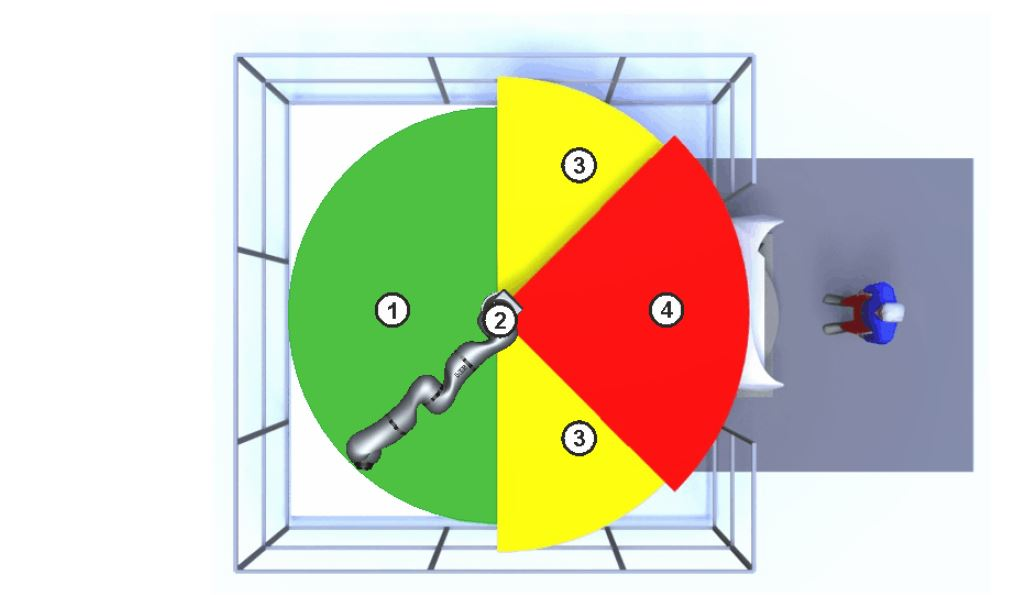
\includegraphics[scale=0.8]{axisrange}
\caption{Példa a mozgástartományokra: 1. munkaterület, 2. beavatkozó, 3. megállási út, 4. biztonsági sáv}
\label{fig:axisrange}
\end{figure}

\subsubsection{Biztonságszempontú funkciók}
Az alábbi funkciók permanensen jelen vannak az ipari robot esetén:
\begin{itemize}
	\item Vészleállító eszköz (\angol{EMERGENCY STOP device})
	\item Engedélyező eszköz (\angol{Enabling device})
	\item Az üzemmód lezárása (a kulcsos kapcsoló által)
\end{itemize}
A következő biztonságszempontú funkciók előre konfiguráltak és a robotvezérlő biztonsági interfészén keresztül bármikor a rendszerbe integrálhatóak:
\begin{itemize}
	\item Üzemeltető biztonsága (= a fizikaileg jelen lévő biztonsági kerítések megfigyelésére alkalmas csatlakozó)
	\item Külső vészleállító eszköz
	\item Külső, útvonalkövető megállást előídéző eszköz (\angol{Stop category 1 (path- maintaining)}) (\ref{tab:terms}. táblázat)
\end{itemize}
Egyéb biztonsági funkciók konfigurálása esetleges, pl.\footnote{A vastag betűvel szedett pontok a szakdolgozat fontos elemei}:
\begin{itemize}
	\item Külső engedélyező eszköz
	\item Tengelyspecifikus munkatér monitorozás
	\item Descartes-i munkatér megfigyelés
	\item \textbf{Descartes-i védett tér monitorozás}
	\item Sebesség nyomonkövetés
	\item \textbf{Tengelyekben ébredő nyomatékok megfigyelése}
	\item \textbf{Üktözés detektálása}
\end{itemize}
Az egyes pontokról további információ a technikai specifikációban található\cite{sunrisemanual}.


\end{document}